\cleardoublepage
\phantomsection 
\addcontentsline{toc}{section}{Prílohy}
\section*{Prílohy}
\begin{enumerate}[leftmargin=*]
    \item Niagara Module Script \label{att:nms}
    \begin{figure}[!htbp]
        \centering
        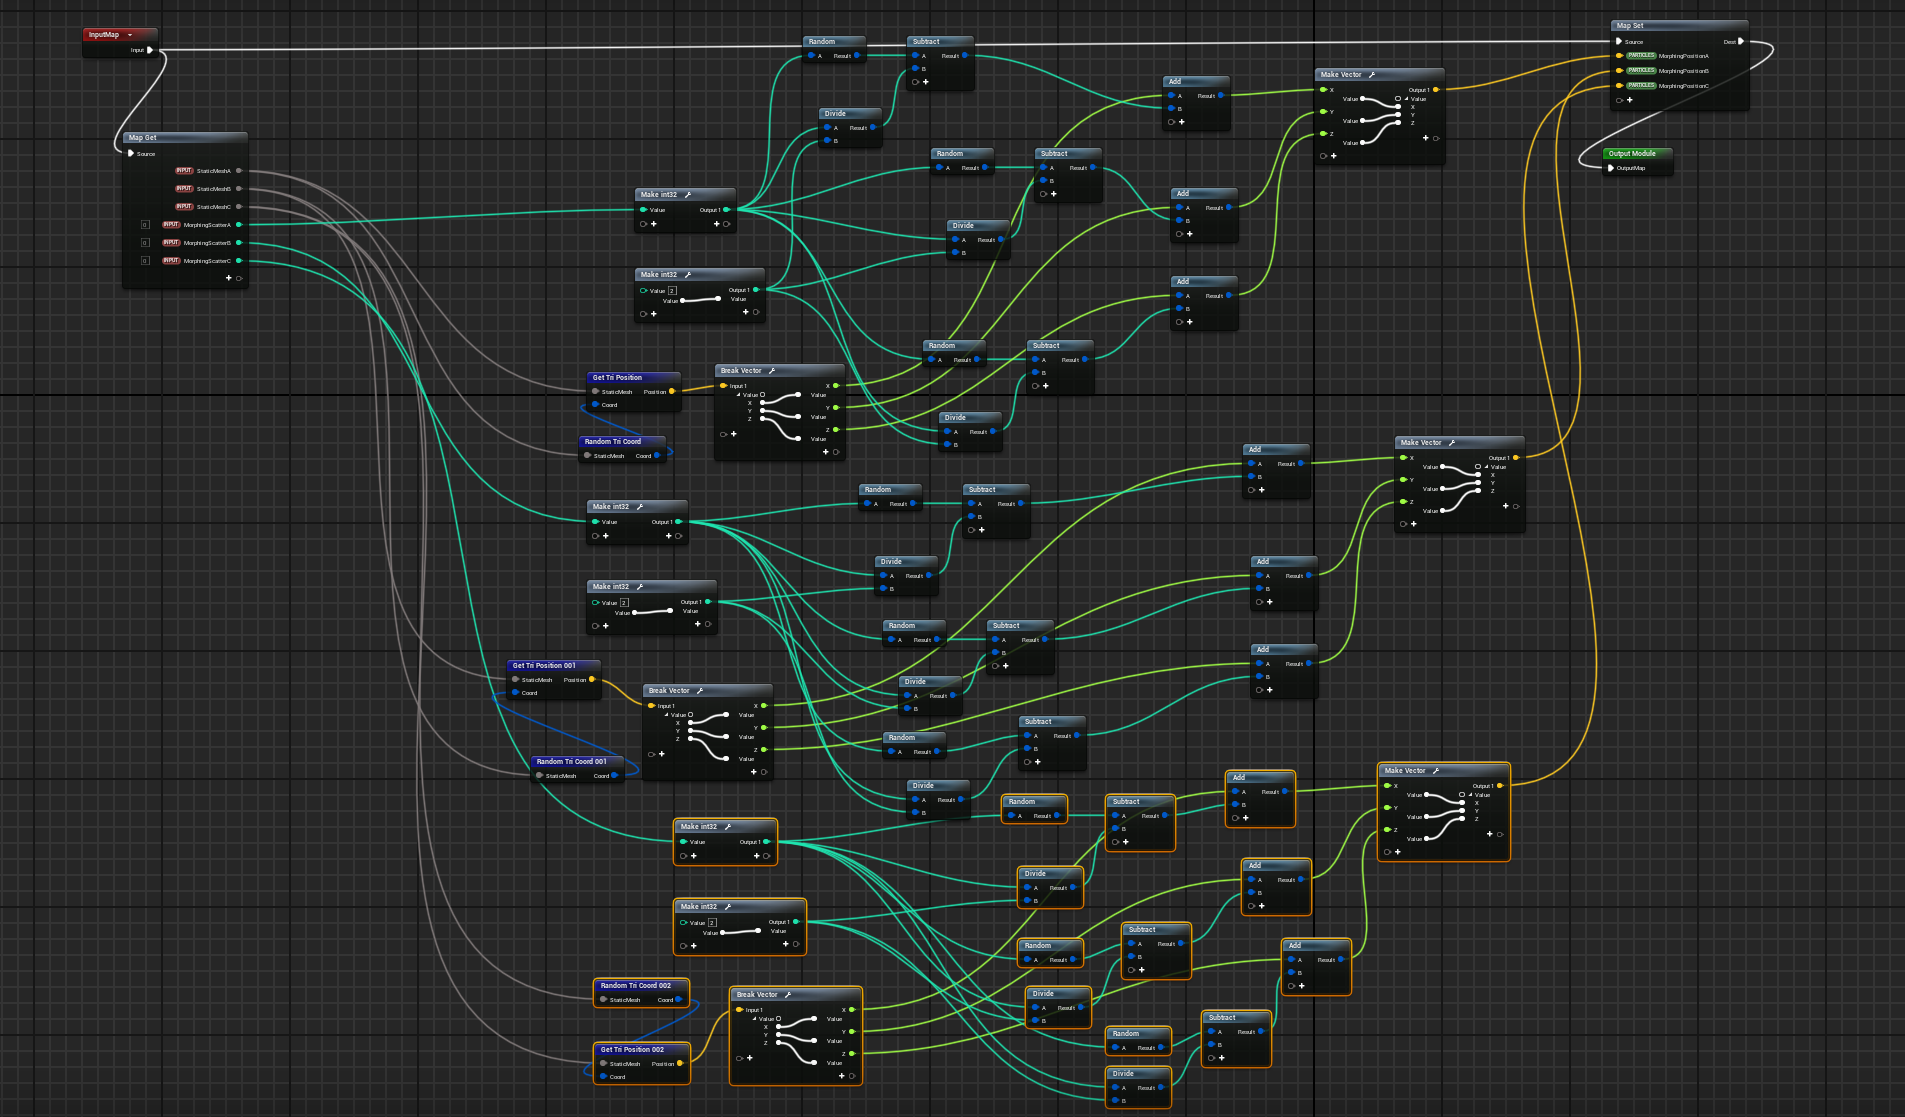
\includegraphics[width=21cm,angle=90,origin=c]{img/nms.png}
    \end{figure}
    \newpage

    \item Blueprint \texttt{Niagara\_3Lerp} \label{att:lerp}
    \begin{figure}[!htbp]
        \centering
        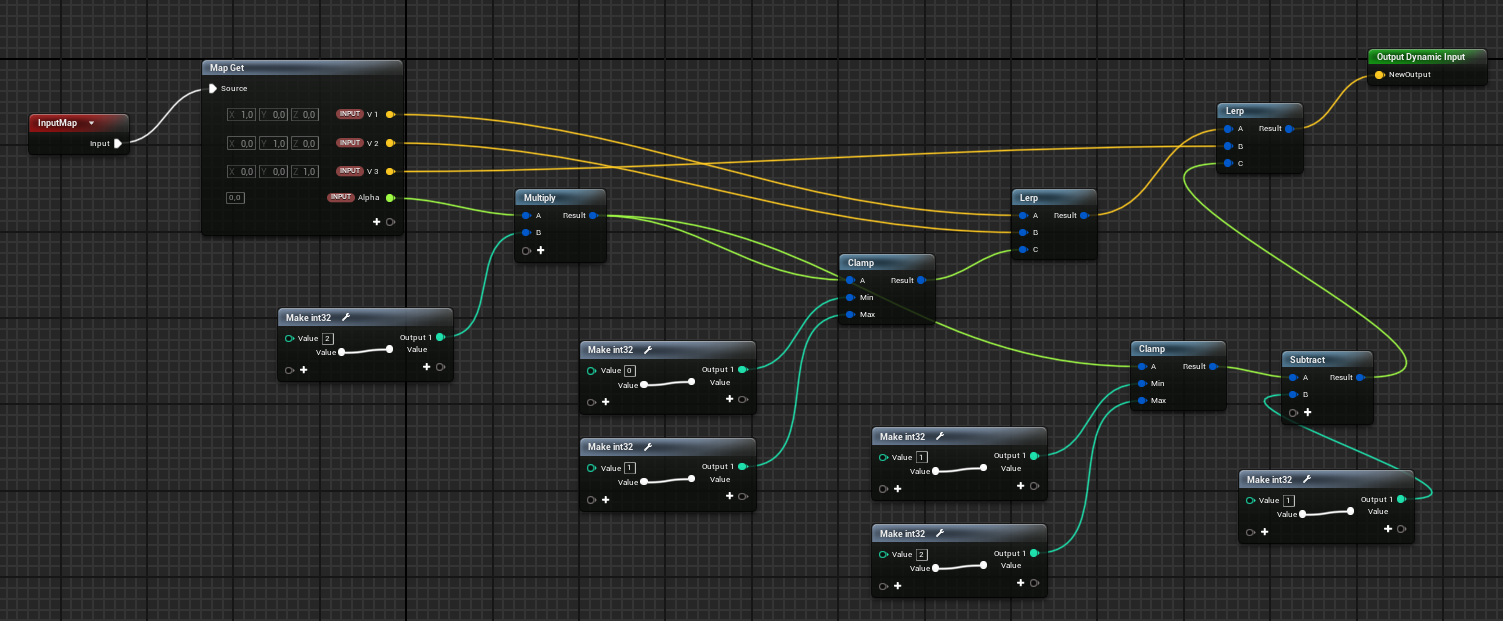
\includegraphics[width=22cm,angle=90,origin=c]{img/3lerp.png}
    \end{figure}
    \newpage

    \item Skript s časovou osou v Blueprinte \texttt{BP\_Neuron} \label{att:main-animate}
    \begin{figure}[!htbp]
        \centering
        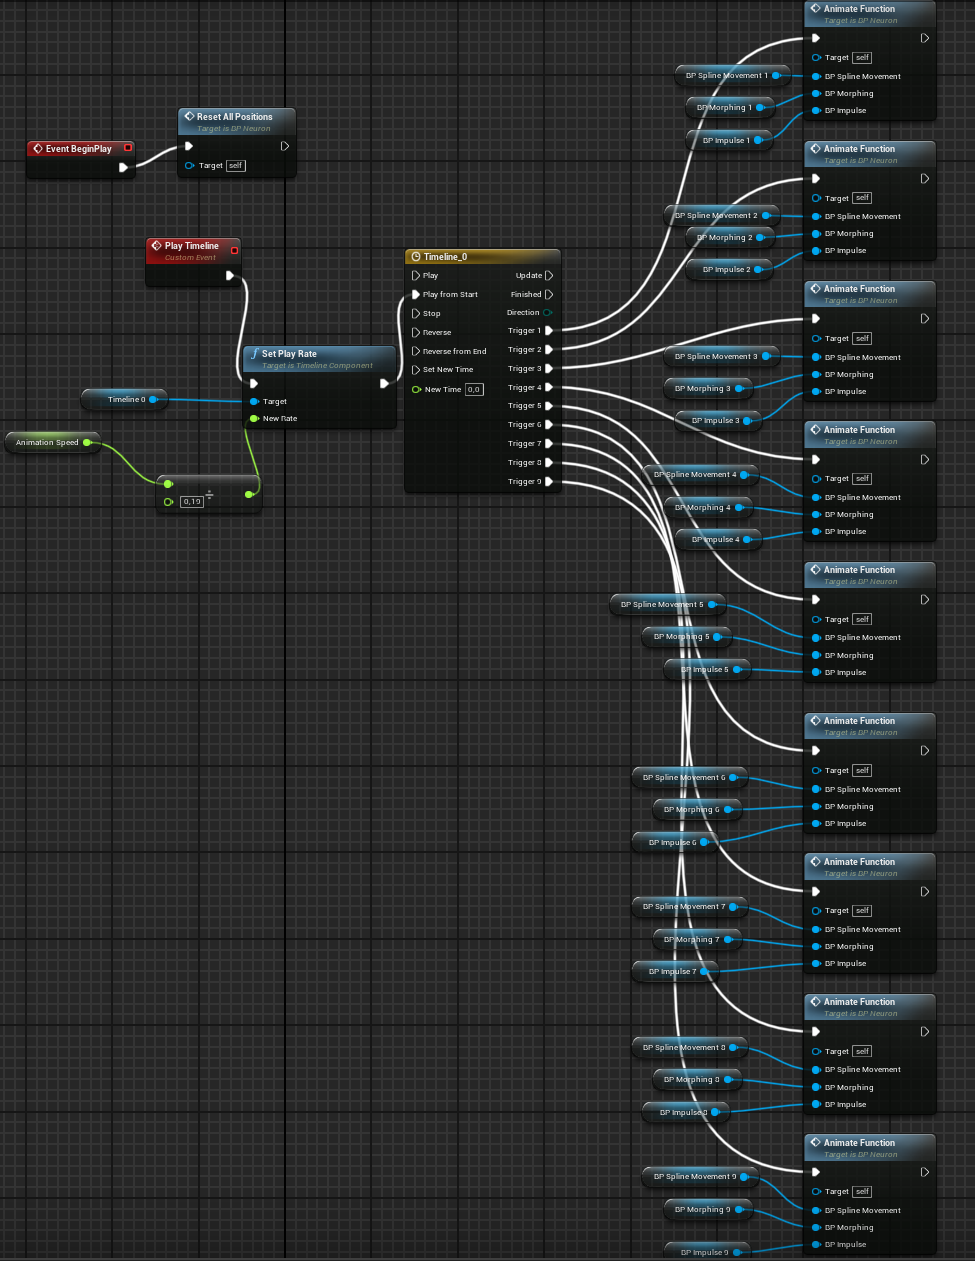
\includegraphics[width=16cm]{img/main-animate.png}
    \end{figure}
    \newpage

    \item Dotazník {--} položky 1 a 2 \label{att:dot1}
    \begin{figure}[!htbp]
        \centering
        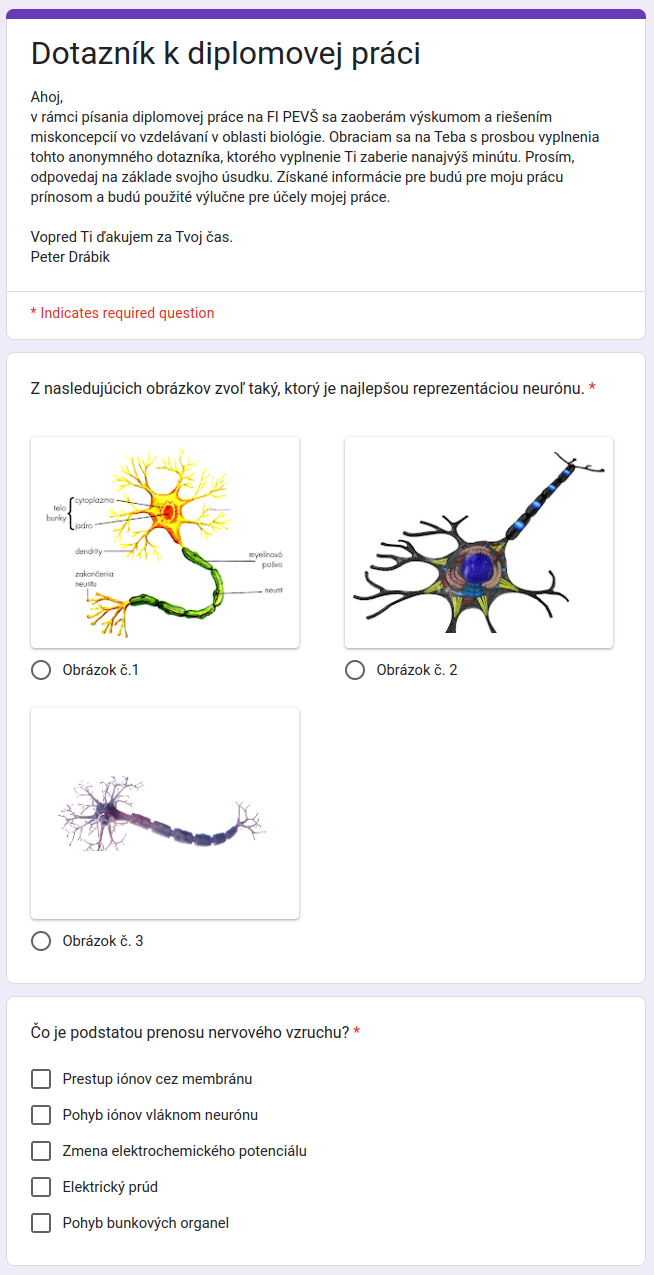
\includegraphics[width=11cm]{img/dot1.png}
    \end{figure}
    \newpage

    \item Dotazník {--} položky 3, 4 a 5 \label{att:dot2}
    \begin{figure}[!htbp]
        \centering
        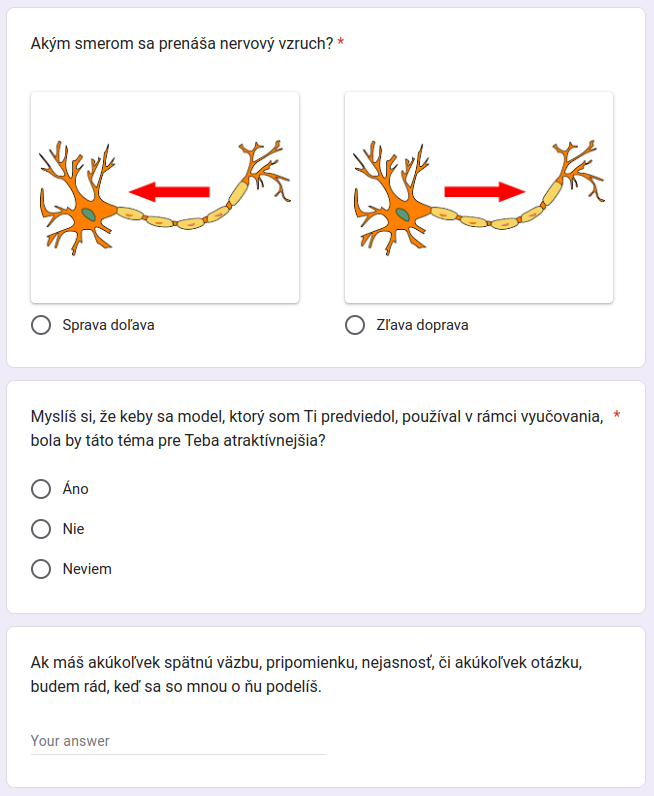
\includegraphics[width=14cm]{img/dot2.png}
    \end{figure}
    \newpage

\end{enumerate}
